\subsection{Long term speckle pulsing}

In experiment, it is important to know the average speckle potential at the atoms. But unfortunately, it is hard to measure the power of the speckle beam directly at the atoms and infer the average speckle potential. Because in experiment, we can not put a power meter anywhere we want. After the closest point to the vacuum glass cell where we can use a power meter to measure the power. The beam goes through lenses, reflected by mirrors, glass cell or even dichroic mirrors. The power of the beam decreases at each of the optical component. To the best of our knowledge, for the previous experiments using speckle beams, the average speckle potential was not measured. It could be inferred by calculating the power given the power loss at each optical component is known. Or the power could be measured for an identical speckle beam set up on the test bench and assume the power at the atoms is the same for the speckle beam used in the experiment. 

Inspired by \cite{huckans2009quantum}, we think the average speckle potential can be measured by evolving the atoms under speckle beam pulses. Compared with \cite{huckans2009quantum}, for $t \gg t_{RN}$, we do not expect to see the collapse and revive phenomenon due to the anharmonicity of the speckle potential. Instead, the at long speckle pulsing time, the momentum distribution should reach equilibrium and by Virial theorem, the average stationary kinetic energy is half of the average total energy which is the initial average speckle potential. 

To confirm our understanding, we did numerical simulation of long-term speckle pulsing. Fig.~ \ref{fig:speckle_pulsing} show the simulation and experimental results of speckle pulsing for pulsing  duration up tp $2 {\rm ms}$. In the simulation, we release the BEC from the dipole trap and immediately turn on the speckle potential. The atoms evolve under the speckle potential and we keep track of the width of the momentum distribution. We did the simulation for different average speckle potential ranging from $0 {\rm Hz}$ to $1600 {\rm Hz}$, with $200 {\rm Hz}$ spacing. The results are shown as the nine curves, each one is averaged over 20 speckle realizations. When the average speckle potential is zero, the width of the momentum distribution increases driven by the mean-field expansion. From the simulation results shown in Fig.~ \ref{fig:speckle_pulsing}(a), the width of the momentum distribution increase rapidly evolving under speckle potential and becomes stationary after around $0.25 {\mu s}$. The stationary width increases with the average speckle potential. Fig.~\ref{fig:speckle_pulsing}(b) shows the experimental results. In experiment, we release the atoms from dipole trap, pulse speckle potential for up to $2 {\rm mm}$ followed by TOF. The time for speckle pulsing plus the time for TOF is fixed, $18 {\rm ms}$. We take absorption images after TOF and fit Gaussian function to the density profile of the atoms in the images. Fig.~\ref{fig:speckle_pulsing}(b) shows the with of the fitted Gaussian function vs speckle pulses duration. The Gaussian width increases with the pulsing duration in short-term and becomes stationary after around $0.25 {\rm ms}$, which is consistent with the simulation results. 

\begin{figure*}
    \centering
    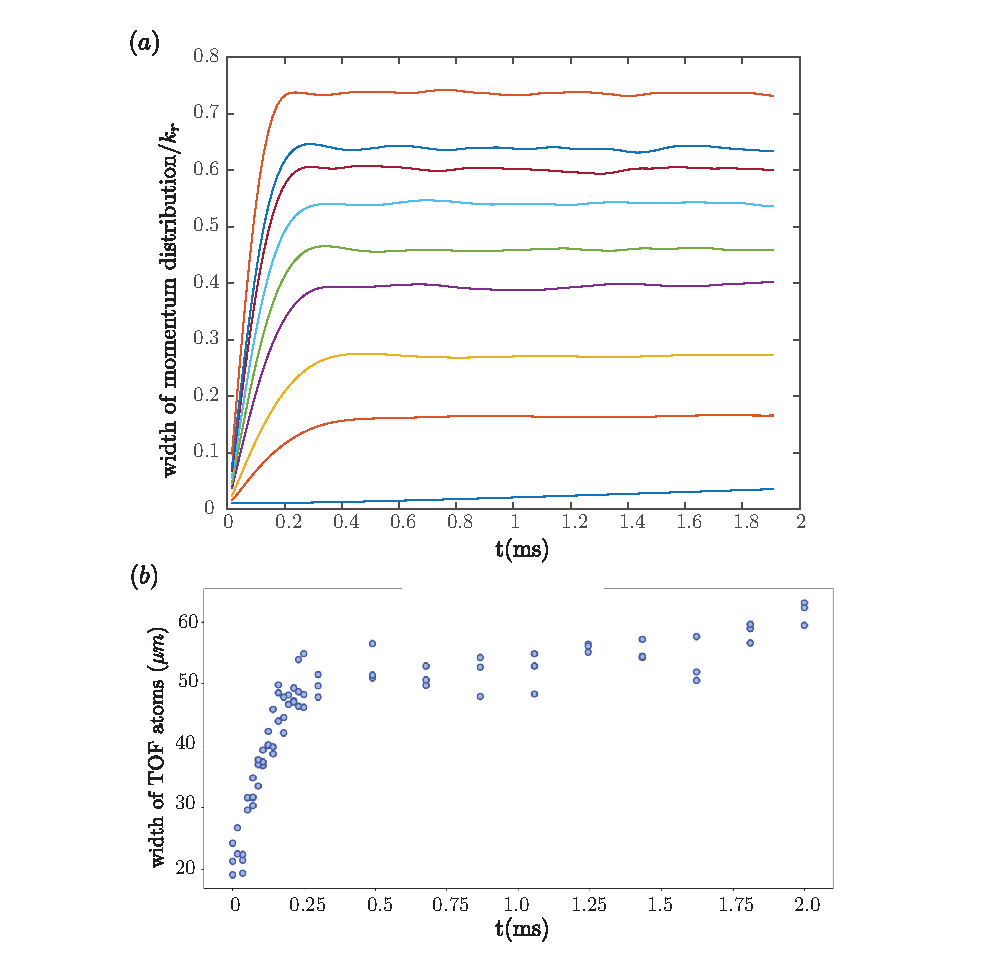
\includegraphics{Chapter6_secs/speckle_pulsing_width.pdf}
    \caption{Simulation and experiment of speckle beam pulsing. (a). Absorption images after TOF for different speckle pulsing time. The width of atoms increases as the speckle pulsing time increases from 0 to $\approx 2 {\rm ms}$. After which the width reaches equilibrium. (b). The Gaussian width of atoms in absorption images for  different speckle pulsing time.}
    \label{fig:speckle_pulsing}
\end{figure*}

To infer the average speckle potential from the width of momentum distribution after long-term speckle pulsing, we compute the average kinetic energy using the fitted Gaussian width of the density profile of atoms after TOF.
\begin{equation}
    \langle \hat{K} \rangle = \frac{1}{2} m \left(\frac{\sigma}{\tau}\right)^2
\end{equation}
Here $\tau$ is the time for TOF. The average speckle potential is equal to the average total energy, which by Virial theorem is twice the average kinetic energy. In Fig.~ \ref{fig:avg_speckle_poten}(b), the computed total energy is plotted against a photo diode (PD) reading. We use a pick off mirror to reflect a fixed percentage of the power of the speckle beam to a PD and the reading of the reading of PD in Volt is proportional to the power of the beam at the atoms. We fit a line crossing the origin to the data, by reading the PD we have an estimate of the average speckle potential at the atoms. 

To compare with the experimental results, we also did numerical simulation. In the simulation, we release the atoms from the dipole trap at $t=0$ and pulse the speckle potential for $1 {\rm ms}$ followed by a $20 {\rm ms}$ free evolution. The simulation is done using two kinds of speckle potentials, $k_c=0.80k_r$ and $k_c=1.48k_r$, respectively. For each speckle potential, the average potential depth ranges from $0 {\rm Hz}$ to $1600 {\rm Hz}$ with a $200 {\rm Hz}$ spacing. We compute the the momentum distribution at the end of TOF and compute the average kinetic energy. The average total energy is twice the average kinetic energy deducted by the average kinetic energy in the no pulsing case. And the resultant average total energy is plotted against the known average potential depth. In agreement with our prediction, the curves are close to the line $y=x$ for both kinds of speckle potentials.


\begin{figure*}
    \centering
    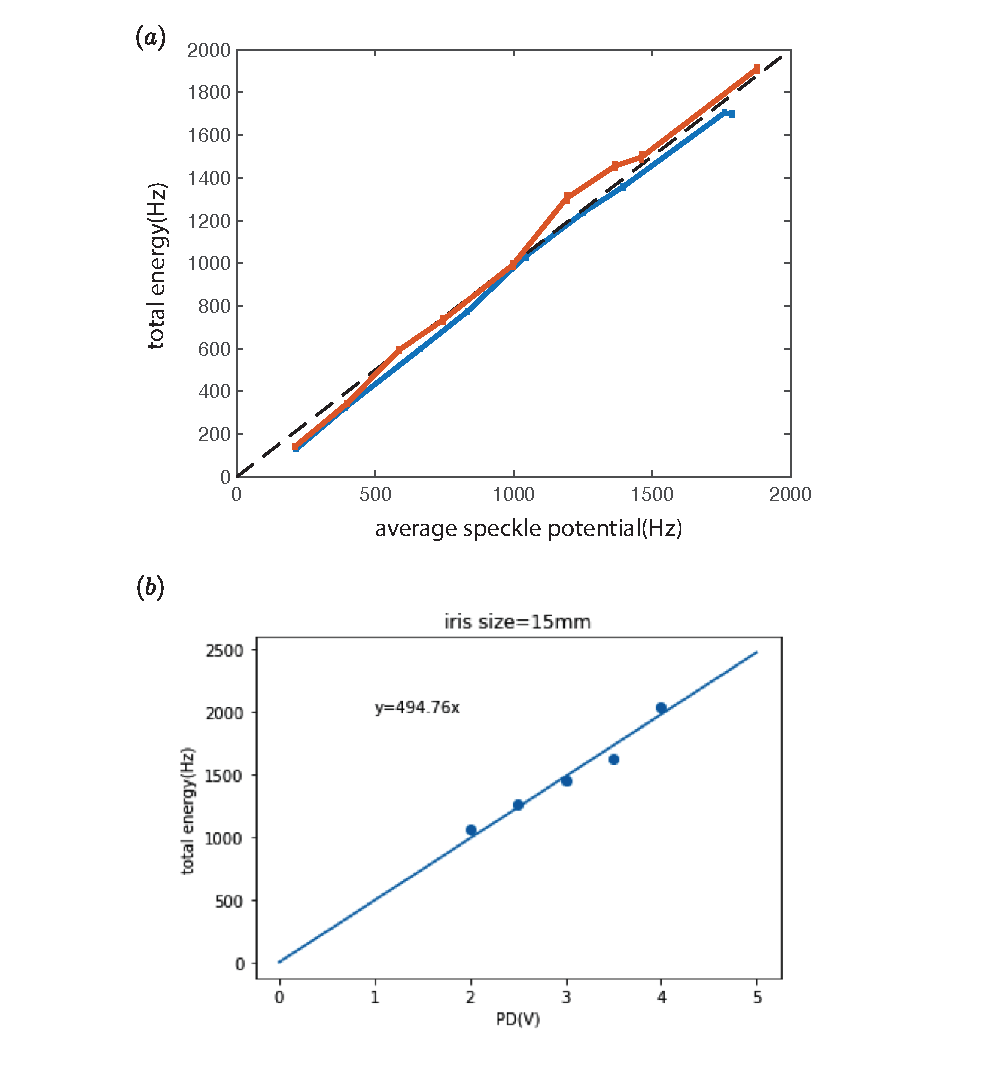
\includegraphics{Chapter6_secs/average_speckle_potential.pdf}
    \caption{s}
    \label{fig:avg_speckle_poten}
\end{figure*}



